\documentclass[12pt, twoside, openright]{report}
\usepackage[french]{babel}
\usepackage{xltxtra}
\setmainfont[Mapping=tex-text]{Linux Libertine O}
\usepackage{amsmath}
\usepackage{graphicx}
\usepackage[colorinlistoftodos]{todonotes}
\usepackage[T1]{fontenc}
\usepackage{titlesec}
\usepackage{url}
\usepackage{hyperref}
\usepackage{geometry}
\usepackage{shorttoc}
\usepackage[backend=bibtex]{biblatex}
\usepackage{caption}

\addbibresource{bibliographie.bib}
\DeclareTextCommandDefault{\nobreakspace}{\leavevmode\nobreak\ } 
\geometry{
    paper=a4paper,
    inner=3cm,
    outer=2.5cm,
    top=2.5cm,
    bottom=3.5cm
}

\setcounter{secnumdepth}{4}

\titleformat{\paragraph}
{\normalfont\normalsize\bfseries}{\theparagraph}{1em}{}
\titlespacing*{\paragraph}
{0pt}{3.25ex plus 1ex minus .2ex}{1.5ex plus .2ex}

\begin{document}

\begin{titlepage}

\newcommand{\HRule}{\rule{\linewidth}{0.5mm}} 
\center
 

\textsc{\LARGE Nanterre université}\\[1.5cm]
\HRule \\[0.4cm]
{ \huge \bfseries Développement d'applications de gestion de projet }\\[0.4cm]
\HRule \\[1.5cm]
 \textsc{\Large Rapport de stage }\\[0.5cm]

\begin{minipage}{0.4\textwidth}
\begin{center} \large
\emph{Auteur:}\\
Baptiste \textsc{rayer} 
\end{center}
\end{minipage}\\[0.5cm]

\begin{minipage}{0.4\textwidth}
\begin{center} \large
\emph{Maître de stage:}\\
 Hamouda \textsc{Raïs} 
\end{center}
\end{minipage}
~
\begin{minipage}{0.4\textwidth}
\begin{center} \large
\emph{Tutrice:} \\
Marta \textsc{Rukoz Castillo}
\end{center}
\end{minipage}\\[4cm]



\includegraphics[width=10cm,height=2.25cm]{img/itnovem2.png}

\includegraphics[width=10cm,height=2.25cm]{img/UPN.jpg}

\vfill 

\end{titlepage}
\renewcommand{\abstractname}{Remerciement}
\begin{abstract}
\begin{minipage}{0.9\textwidth}
\begin{flushright}
\emph{Je souhaite remercier Hamouda, Mohamed, Ophélie ainsi que Selam pour leur soutien apporté durant le stage.}\\

\emph{Je souhaite aussi remercier tous l'entreprise Itnovem pour son accueil.}
\end{flushright}
\end{minipage}



\end{abstract}
\newpage

\shorttoc{Sommaire}{1}

\chapter{introduction}

Mon stage se déroule dans les bureaux de Itnovem. Mon maître de stage est M. \textbf{Hamouda Raïs} et ma tutrice est Mme. \textbf{Marta Castillo Rukoz}. Ce stage se déroule sur une période de 5 Mois à partir du 9 avril 2018. Mon objectif durant ce stage est de créer plusieurs outils de gestion. Le premier est un outil permettant la génération automatique de mails en fin de sprint. Le premier projet m'a permis d'acquérir des connaissances sur plusieurs logiciels de gestion de projet professionnel en manipulant leur API REST. Le second projet a pour but d'automatiser l'envoi et le traitement de mails de satisfaction. Le troisième est un portail pour faciliter le travail des Ressources Humaines de l'entreprise. Ce dernier projet n'a pas encore commencé à ce jour.

\section{Entreprise}

\subsection{Itnovem.}
% * <batrayer77@gmail.com> 2018-05-03T13:58:03.732Z:
% 
% Bon en vrai faudrait demander à une RH de refaire son speach
% 
% 
% ^.
Itnovem. est une filiale technologique de la SNCF. Ils sont responsable de nombreux projets de développement java, php, angularjs et nodejs. Ils travaillent aussi dans le milieu de l'IOT. Il s'agit de l'Internet Of Things, des objets connectés principalement. L'un des projets consiste en un capteur connecté qui permet de détecter si un wagon à besoin d'un ravitaillement en eau. Nous retrouvons aussi l'application qui permet aux utilisateur des trains de signaler des problèmes d'entretiens via un QR Code dans le train. Malgré son importante croissance en effectif, Itnovem se veut ouvert, et pour ce faire, les locaux ressemblent à un open-space géant. Les seuls séparations entre les groupes de projet sont des rideaux.

\subsection{L'équipe php}

Je suis actuellement affecté à l'équipe PHP de l'entreprise. Il s'agit d'une équipe composée de 4 personnes, (Hamouda, Mohamed, Ophélie, Selam) qui travaillent sur des projets innovants tel que MyStarterZen, une application permettant de faire valider ses projets informatiques auprès des Responsables de la Sécurité des Systèmes d'Information (RSSI). Ils gèrent plusieurs projets en même temps et travaillent en méthode agile. 

\chapter{Les missions}

\section{Génération de mail}

La majorité des groupes de projets de Itnovem travaillent en méthode agile. Chaque groupe utilise un outil de gestion de projets. À la fin de chaque sprint, chaque équipe doit rédiger un mail à son client. Cela prend un temps considérable d'écrire ce mail correctement. J'ai donc comme mission de créer un outil récupérant les informations du sprint afin de composer un mail de fin de sprint.

\subsection{Problématique}

Lorsqu’on effectue un projet en méthode agile, le but premier est de développer des fonctionnalités sur un temps relativement court nommé "sprint" ou "itération". À la fin d'un sprint le projet peut être utilisé par le client. Les tâches à effectuer durant un sprint sont déterminées au début du sprint. Toutes les tâches ne sont pas forcément réalisées durant un sprint. Il est donc important de communiquer au client, à la fin du sprint, qu'elles sont les tâches qui ont été implémentées durant le sprint. Pour cela chaque chef d'équipes reprend son projet et rédige une par une les tâches effectuées dans un mail. Ce travail peut prendre pas mal de temps et des fonctionnalités réalisées peuvent être oubliées lors de la rédaction de ce mail. 

La création d'un outil générant les mails de fin de sprint permettrait aux utilisateurs de gagner du temps lors des fins de sprints. De plus, comme le processus serait automatisé, nous pourrions envisager des améliorations à ces mails. Par exemple, ajouter un lien hypertexte qui redirige vers la story disponible dans l'outil qu'utilise l'équipe. Ce petit détail qui est extrêmement pratique pour un Product-Owner prendrait un temps considérable à faire à la main.

\subsection{Contraintes}

Nous avons une contrainte principale durant ce projet. Comme l'application ne va pas contenir qu'un générateur de mail, il faut faire en sorte qu'elle soit adaptable. Le fait de pouvoir ajouter un module à l'application permettrait d'éviter que les employés de Itnovem se retrouvent à avoir plusieurs applications différentes qui n'effectuent qu'un seul travail. Cette application que je vais développer va servir de plate-forme à d'autres applications, et je ne vais pas forcément développer moi-même toutes les nouvelles applications. Il faudrait donc que les développeurs soient capable d'ajouter leurs applications sans effort sur la plate-forme. Pour cela je dois au maximum organiser mon code et respecter les structures des outils que j'utilise (Angular regroupe ses composants par dossier par exemple). Il s'agit ici de la contrainte principale du travail dans Itnovem. 

J'ai reçu une deuxième contrainte plus spécifique à l'équipe à laquelle je suis affecté. Ils travaillent eux aussi sur une plate-forme contenant plusieurs sous applications. Avec la plate-forme que je vais développer nous allons tester de nouvelles pratiques de gestion de projets qu'ils pourront plus tard mettre en œuvre sur leurs projets. Je me retrouverais donc à tester de nouvelles pratiques qui n'ont pas forcément été réalisées auparavant par un  membre de l'équipe. Il faudrait aussi que j'apporte un soin particulier au travail que j'ai effectué durant le projet. Je devrais être capable d'expliquer comment j'aurais obtenu une configuration spécifique par exemple.  

\section{Mail de satisfaction}

Itnovem souhaite récupérer les avis des clients pour chaque projet afin de maintenir une bonne entente avec ses clients. Pour ce faire il faut générer un mail tous les mois qui permet au client d'exprimer leurs satisfactions sur le projet sur lequel ils travaillent. En plus de ce mail, il faudrait réaliser un affichage pour pouvoir consulter les données. 

\subsection{Problématique}

Avec un grand nombre de projets et d'équipes, Itnovem souhaite pouvoir effectuer des statistiques sur les retours clients. Pour ce faire et dans un premier temps, il faut que les clients donnent leurs satisfactions mais interroger chaque client n'est pas envisageable. Ensuite il faut que les clients soient interrogés régulièrement, sinon le nombre de votes ne serait pas suffisant pour pouvoir obtenir des statistiques utilisables. Cependant il faut que les clients aient travaillés sur le projet récemment pour que leurs votes soient comptabilisés. On ne souhaite pas qu'une personne ayant travaillée sur un projet, il y à deux ans, puissent fausser le résultat des votes alors qu'elle n'a pas participé sur ce projet depuis. Comme il s'agit d'une application impliquant une action facultative du client, il est souhaitable que le mail soit le plus agréable à lire. Si le mail n'est pas agréable à lire pour le client il ne donnera que très rarement sa satisfaction. L'équipe design de Itnovem peut nous fournir un modèle de mail mais il faut l'implémenter le mieux possible. Ensuite, il est souhaitable d'avoir un affichage de ces résultats pour des administrateurs.

\subsection{Contraintes}

Nous avons eu plusieurs contraintes pour réaliser cette mission. Notre projet doit être implémenté sur la plate-forme que nous avons créée précédemment, ce qui implique de respecter les contraintes inhérentes à la mission précédente (respect des normes de programmation, du code réutilisable...). Il faut aussi faire extrêmement attention à ce que les mails ne soient pas envoyés alors que les tâches ne sont pas finies. Il ne faudrait pas qu'un client reçoivent un mail avant que le design soit implémenté correctement. 

Cette application de vote se trouvant sur Metrit, le client pourrait avoir accès à toute l'application. Il nous faut donc envisager un moyen d'éviter que les personnes externes puissent accéder au reste du site. Elles devraient avoir accès uniquement au module pour voter et ajouter un commentaire. L'affichage des résultats des votes ne doit pas non plus être accessible au client.

\leavevmode\thispagestyle{empty}\newpage
\leavevmode\thispagestyle{empty}\newpage

\chapter{Metrit}

Metrit correspond au nom de la plate-forme que nous avons développés au cours du stage. A ce jour, la plate-forme contient deux applications principales : 
\begin{itemize}
\item Le générateur de mails de fin de sprint.
\item La métrique de la satisfaction client.
\end{itemize}

\section{Mise en place}

\subsection{La méthode agile}
Comme indiqué auparavant, Itnovem travaille principalement en méthode agile. Nous avons donc décidé de développer Metrit en méthode agile. Pour cela nous avons séparé le travail en plusieurs sprints. Chaque sprint suit le schéma classique de la méthode agile. On débute en définissant les tâches à effectuer pendant cette itération. Quelles sont les tâches qui apportent le plus de valeur au projet ? Cette story est-elle bien rédigée ? Est-elle bien découpée ? Cette réunion prend un certain temps en début de sprint mais est nécessaire afin de ne pas perdre de temps plus tard. Cela évite donc de se retrouver bloqué sur une story voire pire de devoir recommencer cette story parce qu’elle a été mal comprise.

Une fois les stories sélectionnées, nous estimons ces tâches avec Hamouda. Pour l'estimation, nous prenons en compte le maximum de points tels que : 
\begin{itemize}
\item La tâche a-t-elle été déjà réalisée par quelqu'un dans l'équipe ?
\item La tâche est-elle difficile d'un point de vue technique ?
\item La tâche implique-t-elle une technologie que je n'ai pas utilisé ?
\end{itemize}

Le fait de se poser un maximum de questions pendant l'estimation permet de mieux estimer la tâche, mais aussi d'obtenir des éléments de réponse pendant cette estimation. En effet Hamouda étant lead développeur de projet PHP/symphony, il est capable d'apporter des éléments de réponse grâce à son expérience. Il peut recommander des Bundles qui répondent aux besoins des stories. 

Chaque jour nous effectuons un daily meeting le matin afin de voir où toute l'équipe en est. Grâce à ce meeting, tous les membres de l'équipe savent où les autres en sont, sur quelles stories ils travaillent... Si quelqu'un est bloqué, nous discutons des solutions pour le débloquer. 

À la fin du sprint, nous revoyons les tâches effectuées et nous discutons des améliorations possibles ainsi que des problèmes rencontrés. Pourquoi cette story n'a pas pu être finie, quelles ont été les difficultés principales, etc. Ces réunions nous ont permis de mieux estimer les stories pour les sprints suivants. 

\section{La plate-forme Metrit}

Afin de pouvoir développer notre application dans les meilleurs conditions possibles, nous devons commencer par créer une plate-forme solide capable de contenir plusieurs applications. Nous nous sommes orientés vers une structure classique qui consiste en deux éléments principaux. D'un coté le back end, avec une API RESTful, et de l'autre un front dynamique en typescript.

\begin{figure}[h]
\centering
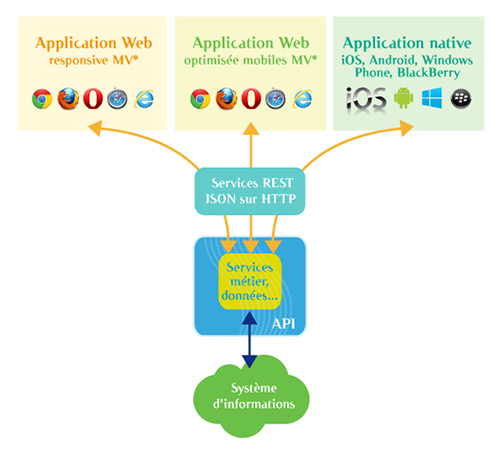
\includegraphics[width=10cm,height=10cm]{img/front-back.jpg}\caption{Schéma de fonctionnement d'un back-front avec une API rest}
\end{figure}



Ce schéma représente comment notre application devrait fonctionner. Dans notre cas, nous allons créer une application Web responsive qui consommera les services de l'API RESTful. L'interface de l'API sera générée par un service dans la partie back end.

\subsection{La séparation Back/Front end}

Cette méthode de création d'application possède plusieurs avantages. Premièrement le code est mieux organisé. Le développeur est obligé de séparer la vue et le modèle. La vue correspond à ce que le client peut observer : une page HTML par exemple. Le développeur ne peux pas créer une vue dans le back end car elle ne sera jamais visible pour le client. De même dans le front end un développeur ne doit jamais avoir a faire une connexion direct à une base de données pour des raisons de sécurité. La séparation entre le modèle et la vue permet notamment un meilleur entretien du code. Il est plus facile de détecter où se trouve la ou les erreurs dans le code.  

Deuxièmement cette structure permet l'ajout d'application front end sans problème. Si une personne souhaite se connecter à notre base de données, il suffit de lui donner l'accès à notre API et consommer nos données sans se soucier d'avoir à écrire des modèles. C'est un gain de temps important pour peu que l'API soit bien documentée. De plus l'application front end peut être de toute sortes (Application android, application web ...).

\subsection{L'API Restful}

Une API Rest correspond à une API disponible par URL. En interrogeant une URL, par exemple "http://www.api-rest.com/api/projets", nous obtiendrons en retour une liste de ressources correspondant au projets. Une API Rest est dites Restful quand elle prend en considération les méthodes du protocole HTML (GET, POST, PUT, DELETE ...). Une API Restful permet de suivre un modèle pour la génération des URLs qui respecte les normes de Rest. L'appel d'une même URL mais avec des méthodes différentes provoquent des résultats différents.

\begin{itemize}
\item GET    /projet Renvoi la liste des projets
\item POST   /projet Créer un projet 
\item GET    /projet/<id> Renvoi le projet en fonction de l'id 
\item PUT    /projet/<id> Modifie le projet en fonction de l'id
\item DELETE /projet/<id> Supprime le projet en fonction de l'id
\end{itemize}

Une API Restful permet donc de mieux organiser ses URLs. Malgré cela il est nécessaire de suivre des normes afin d'avoir une API durable et cohérente. Il existe cependant différentes normes, le point clé est de rester sur une seule et ne pas essayer d'en suivre plusieurs. Une fois l'API déployée et rendue utilisable pour de nouveaux utilisateurs, il n'est pas envisageable de modifier les routes parce qu’elles ne sont pas aux normes. Des utilisateurs verraient leurs applications ne plus fonctionner à cause de la modification de la route. Maintenant que nous avons une meilleure compréhension du fonctionnement des APIs RESTful ainsi que de la séparation entre back end et front end, nous allons parler des outils qui ont permis la conception de Metrit.

\subsection{Symfony le framework back end}

Nous avons choisi Symfony 4.0 comme outil pour développer notre back end application. Il s'agit d'un framework robuste existant depuis 2005. Il bénéficie d'une communauté de plus de 300 000 développeurs (d'après le site communautaire de Symfony). Symfony fonctionne par Bundle. C'est à dire que la communauté (ou pour certains Bundles l'entreprise SensioLab à qui appartient Symfony) peut rajouter des extensions qui facilitent le travail des développeurs. Par exemple le Bundle FriendsOfSymfonyRestBundle (FOSRestBundle) permet de créer une API Rest. 

Nous aurions pu choisir d'autres Framework qui produisent le même résultat tel que SpringMVC, Django ... Mais nous nous sommes orientés vers Symfony 4 pour des raisons pratiques. Les projets sur lesquels travaillent notre équipes sont tous des projets Symfony. De plus la version 4 permet d'anticiper sur des futures mise à jour. Grâce à Metrit l'équipe PHP peut découvrir de nouvelles fonctionnalités de la version 4, ce qui sera utile quand les projets en cours devront être mis à jour à cette version de Symfony. 

Pour faire fonctionner Symfony comme nous le souhaitions, nous avons dû installer plusieurs Bundles principaux. Le premier : \href{https://symfony.com/doc/current/doctrine.html}{\textbf{Doctrine}}, est un Bundle permettant de faire de l'ORM. La base de données est écrite en PHP et traduite en SQL par Doctrine. En plus de cette génération de base de données, Doctrine permet à son utilisateur de créer des migrations. Cela permet de maintenir la base de données à jour sur tous les environnements. Elle permet aussi de créer des classes Repository qui permettent de générer des requêtes SQL. Avec ces Repository il est beaucoup plus dificile pour une personne tierce de faire de l'injection SQL, du code SQL n'étant pas exécuter directement en PHP. 

Le second Bundle principal est \href{https://symfony.com/doc/current/bundles/FOSRestBundle/index.html}{\textbf{FOSRestBundle}}. Il s'agit d'un outil permettant de créer des vues, des contrôleurs et un système de routing pour une application Symfony. Les vues crées par ce Bundle correspondent à des pages JSON. 

\subsection{Angular pour le front}

Nous avons choisi Angular 5 en tant que framework front end. Angular 5 est un framework typescript possédant une importante communauté et à été développé par Google. Il s'agit donc d'un framework robuste et parfaitement entretenu. Durant ce stage Google à d’ailleurs sortie une nouvelle version majeure d'Angular. 

A nouveau, il existe beaucoup de framework front possible. ReactJS ou VueJS auraient pu faire le même travail qu'Angular. Le facteur décisif fut le fait que la majorité des applications "front" de Itnovem ont été réalisées en Angular. De plus je possède les connaissances de base d'Angular ayant déjà réalisé un projet sous une version antérieur d'Angular. 

\subsection{Docker}

Afin d'avoir le même environnement de développement que l’environnement d'intégration et de production, nous travaillons avec Docker.

Docker est un outil permettant de créer des containers. Chaque container agit comme une petite machine virtuelle consommant un minimum de ressources pour exécuter ses tâches. Chaque container est isolé, c'est à dire qu'il n’interagit pas avec son environnement. Qu'un container se trouve sur Windows, Linux ou Mac, il aura le même comportement. Bien entendu les containers peuvent communiquer entre eux avec un minimum de configuration. Si le docker contenant la base de données ne pouvait pas être utilisé par le docker contenant le back end cela ne servirait à rien. Docker recommande de plus la séparation des tâches. Comme expliqué précédemment, avoir plusieurs container docker permet de faciliter le déploiement du projet sur l'intégration et la production.  

%met les cinq containers sous forme de liste
Nous avons eu besoin de 5 containers pour ce projet.
\begin{enumerate}
\item Le container contenant l'application PHP. Il à pour but de faire fonctionner symfony et tous ses outils.
\item Le container contenant le serveur Nginx. Il permet de réaliser la configuration d'un serveur Nginx. Ont retrouve par exemple la mise en place d'un reverse proxy pour rediriger l'utilisateur.
\item Le container contenant la base de données sql.
\item Le container 'mail\_catcher' qui permet d'intercepter l'envoi de mail. Il est important dans le développement de l'application car cela évite d'envoyer des mails, mais permet aussi de voir le mail que va recevoir le client.
\item Le container PHPMyAdmin contient l'application PHPMyAdmin. Cette application permet d'avoir une vue rapide de la base de données.
\end{enumerate}

Nous pouvons retrouver sur le site de docker des images pré construite de container permettant de travailler directement avec un container entretenu par la communauté. Par exemple, le container php:7-fpm possède une version à jour de php 7. Malgré cela nous avons besoin de modifier le docker, par exemple pour indiquer le proxy de l'entreprise ou pour installer un package particulier à nos besoins. Pour cela nous avons créer un Dockerfile contenant tous nos paramètres d'installation. 

\subsection{Apprentissage des technologies}
% il y a des phrases redondantes dans ce paragraphe que tu pourrais retirer
N'étant pas familier avec Symfony il m'a fallut apprendre cette technologie. Il y a plusieurs points notables que j'ai découvert. Le travail avec les Bundles est l'un d'entre eux. Il s'agit d'une habitude que je n'avais pas auparavant. Mais avec Symfony, il est recommandé d'utiliser les Bundles des autres développeurs. En plus de gagner du temps sur le développement, un gain supplémentaire se fait sur l'entretien. Si le Bundle n'est pas modifié en plusieurs années, l'installateur de Bundle le considère comme déprécié et recommande des alternatives à celui-ci. À tout moment nous pouvons installer les mises à jour et découvrir quels Bundles sont dépréciés grâce à cet installateur.

Ayant déjà fait de l'Angular 2 je possède des facilités pour apprendre Angular 5. De plus, il ressemble beaucoup à React qui est un framework que j'ai utilisé pour mon projet de master. J'ai remarqué que comme pour Symfony les Bundles ont pris de l'importance dans Angular comparé à ce dont je me souvenais avec Angular 2. 

\section{Générateur de mail de fin de sprint}

\subsection{Étude de l'existant}
L'idée d'un générateur de mail relève d'un besoin interne de l'entreprise. Beaucoup d'entreprises devraient avoir le même besoin. Mais malgré cela on ne retrouve que peu d'informations sur le net. Il n'y a d'ailleurs aucun projet de ce type sur Github. Ce qui s'en rapproche le plus sont les outils de gestion de projet tel que Jira, Trello, IceScrum. Ces outils permettent la gestion de projets complète. Ils sont d'ailleurs utilisés par les membres de Itnovem. 

\subsubsection{Trello}

Trello est un outil permettant de gérer des tâches. Sa base est extrêmement simple il contient des cartes qui représentent des tâches à effectuer. Ces cartes se trouvent dans des listes. Ces listes peuvent représenter absolument tous ce que l'utilisateur peut imaginer. Ces listes sont elles-même contenues dans un tableau. Et ces tableaux peuvent appartenir à des groupes d'utilisateur. On peut donc facilement imaginer comment faire un projet agile à partir de Trello. À chaque fois qu'un utilisateur modifie une carte, la déplace ou bien l'archive, tous les utilisateurs qui suivent celle-ci reçoivent un mail de notification. La même chose est valable pour une liste et un tableau. Une personne peut suivre ce qu'il souhaite. Il est donc parfaitement envisageable en fin de sprint lorsque l'équipe de projet finie son sprints qu'elle archive la liste "terminé". Ainsi les clients recevront la notification et pourront consulter à partir de cette notification quelles cartes ont été réalisées. 

Trello est un outil fortement paramétrable. Il est ouvert à tous le monde et il ne limite quasiment pas l'utilisateur. Il existe même des plugins pour modifier Trello en outil de gestion de projet agile. Par exemple \href{https://chrome.google.com/webstore/detail/scrum-for-trello/jdbcdblgjdpmfninkoogcfpnkjmndgje}{\textbf{Scrum for Trello}} permet entre autre aux utilisateur d'affecter un effort au taches. Il s'agit d'ailleurs d'un des plugins que nous avons utilisés pendant ce stage. Trello est tellement modifiable qu'il n'est pas reconnaissable entre deux projets. Cela peut compromettre l'automatisation d'actions via des scripts. Pour réaliser Metrit sur cet outil de gestion de projet il faudrait que tous les membres de Itnovem travaillant sur Trello applique les même méthode de travail, les même outils etc ... Une autre solution serait d'utiliser ou de créer un plugin pour Trello spécifiquement. Ce plugin aurait pour but de normaliser les tableaux. Il s'agira peut être d'un future projet pour l'entreprise.   

\subsubsection{IceScrum}

IceScrum est un outil de gestion de projet agile en scrum. Il est l'outil utilisé par l'équipe PHP sur leur projet principal. Il permet de planifier des sprints, de créer des stories, de les évaluer ... Il s'agit d'un outil complet pour le gestion des projets agiles. Il n'est pas extrêmement personnalisable. Son objectif principal est de faciliter le travail du Scrum master.

IceScrum envoie une notification le jour de la fin du sprint aux utilisateurs. Cette notification correspond uniquement à un message annonçant la fin du sprint. Aucune précision n'est ajoutée. Les développeurs travaillant sur le projet doivent donc récupérer les stories terminées pour les envoyer aux clients.

\subsubsection{Jira}

Jira est lui aussi un outil de gestion de projet. Tous comme IceScrum il est spécialisé dans les projets agiles scrum mais il possède néanmoins la gestion de projet par kanban. Un projet par kanban ne correspond pas vraiment à une pratique agile. Une seul équipe travail ainsi chez Itnovem. Cela correspond principalement à un flux continu de tâche. Lorsque le client a une story, il l'ajoute au tableau. Les développeurs travaillent donc sans sprint. Ce projet de Itnovem ne peut donc pas marcher avec notre outil vu qu'il ne possède pas de sprint.
% tu dis que l'equipe qui utilise jira ne fait pas de sprint et apres tu dis que tu peux cloturer les sprints 
Mais comme indiqué précédemment, une seule équipe travaille avec le projet Kanban. Les autre équipe utilise le mode scrum de Jira. Ce mode de Jira possède un bouton qui clôtures les sprints. Ce bouton envoi un message aux utilisateurs sur ce projet. Ce message ne contient qu'un texte expliquant que le sprint à été clôturés puis il modifie le statut du sprint dans la base de donnée en : "fini". Nous n'avons pas la main sur le mail qui est envoyé. 

\subsubsection{Conclusion de l'existant}
% mail de fin de sprint à répétition
Si un projet permettant de générer des mails de fin sprint existe, il n'est pas disponible en ligne. Les outils couramment utilisés par l'Entreprise ne bénéficient pas de configuration pour les mails de fin de sprint. Jira et IceScrum envoient tous les deux un mail mais il n'est pas précis. Trello quand à lui est spécial dans son interaction. Pour envoyer un mail il faut effectuer des actions spécifiques qui ne sont pas intuitives. Au final le plus simple avec ces outils est de rédiger soi-même ces mails. Une automatisation de la rédaction de ces mails est donc envisagé. Mais afin de pouvoir réaliser l'application, une étude sur la faisabilité du projet est nécessaire. 

\subsection{Étude de la faisabilité}

Metrit à pour but d'être utilisé par un maximum de groupes dans l'entreprise. Le premier travail à faire est de se renseigner sur les outils employés par les groupes de projet. Nous avons donc notés plusieurs outils de gestion de projet :

\begin{itemize}
\item Icescrum
\item Jira  
\item Trello 
\item MantisBT
\end{itemize}

Nous avons pu déterminer la faisabilité de Metrit sur les 2 premiers outils. En effet Icescrum bénéficie d'une \href{https://www.icescrum.com/documentation/rest-api/}{\textbf{API Restful}} basique CRUD (Create, Read, Update, Delete) pour la version utilisée par l'équipe. Jira bénéficie aussi d'une \href{https://developer.atlassian.com/cloud/jira/platform/rest/}{\textbf{API Rest}} mais avec beaucoup plus de fonctionnalités et de contrôle sur les données.

Trello possède une \href{https://trello.readme.io/docs/api-introduction}{\textbf{API Rest}} complète ainsi que des Webhook (Lors d'un changement de données Trello peut envoyer une requête sur un serveur grâce au Webhook) si besoin. Mais comme expliqué précédemment, Trello est trop modifiable pour pouvoir créer un outil générique. D'un groupe à l'autre les données ne seront pas récupérable correctement. Par exemple une équipe peut utiliser un tableau par sprint alors qu'une deuxième équipe peut utiliser des listes pour les sprints.

MantisBT possède deux APIs utilisables : une API REST et une API SOAP. Le groupe de l'entreprise utilisant MantisBT sont actuellement à une version legacy. Cette version permet uniquement l'utilisation de l'api SOAP. Mais dans un \href{https://support.mantishub.com/hc/en-us/articles/203574999-MantisHub-SOAP-API}{\textbf{message récent sur leurs blog}} ils annoncent la fin de cette API qui est déjà dépréciée depuis un certain temps.

Nous décidons donc de commencer par travailler uniquement sur IceScrum ainsi que Jira.

\subsection{Réalisation}

Le schéma qui suit représente comment fonctionne notre application. Le back end récupère les données depuis la base de données ou depuis Jira/IceScrum. Les contrôleurs et services traitent les données puis renvoient une vue JSON. Le front end consomme cette vue puis en génère une nouvelle pour le client. 

Le service \href{https://github.com/csarrazi/CsaGuzzleBundle}{\textbf{CSAGuzzle}} correspond à un Bundle Symfony. Il permet la création de requêtes HTML vers d'autres sites. Nous préférons utiliser cet outil, car il permet de configurer facilement des "Clients". Ces "Clients" correspondent à des sites vers lesquels nous allons envoyer des requêtes HTTP. En injectant le service dans une classe, nous avons accès aux "Clients" configurés auparavant et ainsi nous pouvons donc envoyer des requêtes HTTP rapidement vers ces Clients.

\begin{figure}[h]
\centering
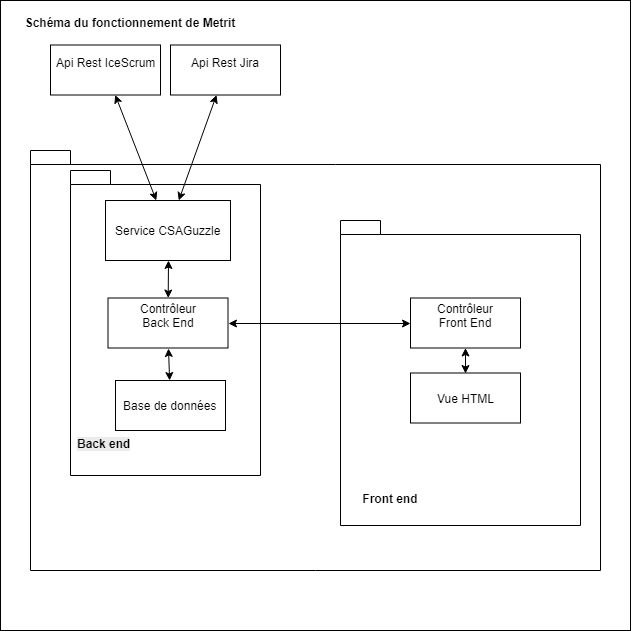
\includegraphics[width=15cm,height=15cm]{img/Metrit.png}
\caption{Schéma du fonctionnement de notre application}
\end{figure}

\subsubsection{Back end}

Dans un premier temps nous avons travaillé sur le back end. Le back end avait plusieurs rôles dans notre application. L'un d'entre eux fut de créer une base de données évolutive. Comme nous travaillons en agile, nous n'avons pas besoin de créer, dés le début, une base de données complète. Il n'est pas nécessaire de générer une classe dans la base qui ne va pas être utilisée pendant les premiers sprints. Nous avons donc créé uniquement les classes qui nous sont utiles au moment où elles le sont. Cette base de données s’agrandit au fur et à mesure que les besoins se font ressentir dans les sprints. 

Ensuite il a fallut faire le lien avec les applications Jira et IceScrum. Pour IceScrum un membre de l'équipe PHP m'a fournit un token de connexion à l'API. Pour Jira j'ai demandé la création d'un compte ayant des droits suffisants pour avoir accès à tous les projets de Itnovem. Cette demande à donc ralentie le développement de l'application.%reformule pour dire que ca a ralentit le dev de l'appli 

Le troisième point important de de ce back end est de rendre consommable les données. Il nous faut pour cela générer des routes qui renvoient des vues JSON contenant les données. Une réflexion importante doit être faite sur le routing. Le respect d'une seule norme est important. Plus récemment un mail reçu nous invite à respecter un nouveau type de norme. Cela provoque donc une dette technique. Il faudra revérifier les routes et voir si elle correspondent au normes envoyées dans ce mail, puis si besoin les mettre à jour. 

Plusieurs problèmes se sont additionnés durant la création du back end lors de l'utilisation des API Rest de Jira et d'IceScrum. Pour IceScrum, leurs API est extrêmement pauvre en données. C'est â dire que pour récupérer les "user stories" finies durant un sprint, j'ai besoin d'effectuer plusieurs requêtes vers l'API REST. Il faut récupérer la liste de tous les sprints afin de récupérer l'id du sprint sur lequel on souhaite générer le mail. Il faut ensuite interroger l'API avec cet id de sprint pour obtenir la liste des user stories du sprint. Cette liste ne contient que les id des user stories. Après toutes ces requêtes effectuées il faut encore une requête pour récupérer les détails de chaque user stories du sprint. Ce grand nombre de requêtes prend un temps important à s'effectuer (3-7 secondes).  

Pour palier à ce problème nous avons essayé de séparer les requêtes en stockant les informations sur le front. Cela permet de limiter la répétition des requêtes. Malgré cela, la récupération de tous les user stories d'un sprint reste longue (3-5 secondes).

Dans le cas de Jira le problème est plus pernicieux. Leur documentation n'est pas claire. On retrouve la documentation sur deux endroits de leur site web. Ces deux documentations ne sont pas identiques. Elle fournissent chacune des données différentes. Seulement l'une d'entre elles donne un moyen d'obtenir des sprints. Il faut donc jongler entre leur documentations. 

\subsubsection{Front}

La création du front n'est pas complexe. Le point le plus compliqué est de faire une interface propre pour que les utilisateurs aient envie d'utiliser Metrit. 

Avec Angular, le site est séparé en composants. Chaque composant contient un contrôleur, une vue et un fichier de configuration. Le fichier de configuration est généré automatiquement par Angular, donc il n'y a pas besoin de s'en soucier. Afin de rendre le code plus facile à entretenir, nous avons séparé cette application en plusieurs composants. Deux composants de vue qui sont globaux à Metrit (deux barres de navigations) et 5 composants spécifiques à ce projet. Avec ces composants, deux services ont été créés afin de se faciliter le travail.

Le premier service est un routeur. Il a pour but de déterminer sur quelle application, en fonction de l'URL, l'utilisateur va être redirigé. Il s'agit d'un service qui est bien décrit par la documentation d'Angular. Avec quelques modifications pour des besoins personnels, nous pouvons facilement rediriger l'utilisateur vers les composants de vue qu'il souhaite observer. Ce service permet aussi, si besoin est, de créer des URLs paramétrées.

Le deuxième service est tout aussi simple. Il s'agit d'un service permettant d'envoyer des requêtes vers le back end Symfony. Il s'occupe de paramétrer les requêtes, de les écrire au bon format et de les envoyer. Ce service utilise le système de variable d'environnement de Angular pour paramétrer l'URL du back end. L'URL est différente entre l'environnement de production, d'intégration et de développement. Il n'est pas vraiment envisageable de modifier le code entre tous les environnements. Le risque d'oubli est trop important et cela peut faire perdre un temps considérable. 

Les composants quant à eux sont principalement des vues. 3 d'entre eux sont des sous vues contenant des formulaires pour choisir les sprints/projets ou bien les détails du sprint. Le quatrième composant génère le mail du côté front et l'affiche dans un \href{https://github.com/Sibiraj-S/ngx-editor}{\textbf{éditeur de texte WYSIWYG}} (What You See Is What You Get). Cela permet à un utilisateur de pouvoir modifier le mail comme il le souhaite avant de le copier/coller vers Outlook pour l'envoyer. Le mail est généré en fonction d'un modèle pré-défini. Ce mail nous donne la vélocité du sprint c'est à dire la complexité en points de toutes les tâches réalisées dans le sprint. Il affiche ensuite la liste des stories réalisées au cours du sprint. Chaque story possède un lien hypertexte vers sur IceScrum ou sur Jira. Nous pouvons trier les stories des IceScrum en fonction de leur feature, c'est à dire en fonction de quel sous projet elles appartiennent. Pour Jira, nous n'avons pas encore réussis à les trier. Le cinquième composant représente une sorte de plate-forme pour les 4 autres composant. Il met en attente l'utilisateur le temps que les données chargent.

\begin{figure}[h]
\centering
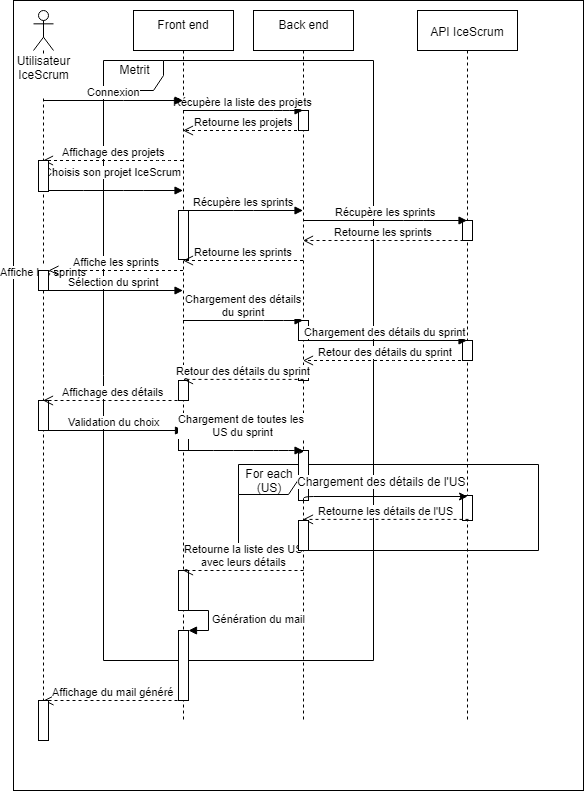
\includegraphics[width=15cm,height=15cm]{img/Diagramme-de-sequence.png}
\caption{Diagramme de séquence de la génération d'un mail d'un projet IceScrum}
\end{figure}

\subsection{Amélioration possible}

Cette application est améliorable. Comme expliqué précédemment, nous ne trions les user stories uniquement pour IceScrum. Grâce à la discussion avec le responsable Informatique, nous pouvons rechercher des solutions du côté des epics pour trier les stories sur Jira. 

Un deuxième axe d'amélioration pour l'application est la création d'un support pour Trello. Cela peut être relativement long mais en discutant avec toutes les équipes de Itnovem, nous devrions être capable de lister comment chaque projet est géré et personnaliser le générateur de mail pour chaque projet. Il est probable que plusieurs projets aient le même fonctionnement ce qui nous arrangerait. Cette amélioration prend trop de temps à implémenter, elle est donc en suspens tant que des tâches apportant une plus grande valeur à Metrit sont en cours.

Sur la documentation d'IceScrum, il est décrit que leurs API REST continuera à évoluer. Il peut être intéressant de consulter les changements de leurs API de temps en temps. Cela permettra un jour de remplacer la boucle qui récupère toutes les user stories par un seul appel à leurs API.

Une solution temporaire à ce problème serait de précharger les données du sprint. En préchargeant la validation de l'utilisateur nous devrions gagner un peu de temps pour améliorer l’expérience utilisateur. Un problème survient avec cette pratique. Si l'utilisateur se trompe une ou deux fois en essayant de sélectionner le sprint, il y a un risque de dépasser le nombre de requêtes par secondes possible pour l'API d'IceScrum. Cela aura pour effet de bloquer le compte utilisateur pendant un certain temps. 

\section{Métrique de la satisfaction client.}

Maintenant que nous avons un rédacteur de mail de fin de sprint, nous souhaitons pouvoir envoyer tous les mois un mail de satisfaction au client. Beaucoup d'entreprise le font, et cela permet de découvrir quels sont les services qui mérites une attention particulière. Ce que nous souhaitons, c'est envoyer un mail mensuel et pouvoir observer les données sur Metrit.

%% A revoir comme intro %%
\subsection{Étude de l'existant}

\subsubsection{Les mails avec Symfony}

Symfony bénéficie d'un excellent outil pour envoyer des mails: \href{https://symfony.com/doc/current/email.html}{\textbf{SwiftMailerBundle}}. Il s'agit d'un Bundle permettant de créer des mails et de les envoyer via Symfony. En configurant les variables d'environnements, et en utilisant un compte SNCF, nous pouvons envoyer des mail depuis le serveur. Cet outil prend une vue "twig" de Symfony comme modèle de mail. Cet outil fait la majorité du travail pour nous. Là où la fonction mail de PHP ne permet que d'envoyer un String en tant que message, SwiftMailer permet d'envoyer une vue, ce qui est beaucoup plus facile à préparer. 

\subsubsection{La tâche cron}

Cron est un \href{https://doc.ubuntu-fr.org/cron}{\textbf{package unix}}, qui permet d'effectuer des tâches à un certain moment. Il s'agit d'un script qui tourne en arrière plan de la machine et qui consomme peu de ressources. Avec un minimum de paramétrages, il permet d'effectuer une tâche tous les premiers jours du mois. Avec cet outil, nous avons donc un moyen d'envoyer tous les mails tous les mois aux membres des projets. Cela permet d'éviter à une personne de devoir effectuer l'envoi de mail à tous les autres. Un fichier crontab se sépare en deux parties principales. Le premier correspond aux paramètres de date et le second à une commande Shell à effectuer. 

Cron prend en paramètre 5 nombres dans un fichier. Ces chiffres correspondent à la minute, l'heure, la date, le mois et le jour de la semaine. Ainsi : "0 12 1 */1 *" Exécutera une commande à 12h00 le premier du mois. */1 Correspond à tous les mois. Le dernier * valide l'envoi du mail peu importe le jour de la semaine (dimanche, lundi...). 

Une fois la date d’exécution de la tâche configurée, il reste à écrire une commande permettant d'envoyer les mails depuis Symfony. Pour cela Symfony peut nous aider.

\subsubsection{Les commandes Symfony}

Symfony vient avec son propre \href{https://symfony.com/doc/current/console.html}{\textbf{système de commandes}}. Certains Bundles l'utilisent fortement, par exemple Doctrine utilise ce système pour permettre à l'utilisateur de générer des classes ou bien d'effectuer des migrations. C'est un outil pratique pour tous les programmeurs. 

Mais Symfony fournit aussi la possibilité de rédiger ses propres commandes. En écrivant nos commandes nous pouvons donc les exécuter dans le Shell. Ainsi nous pouvons obtenir une commande Shell qui permet l'envoi de mail à tout un groupe de personnes. Cette commande peut donc être effectuée par une tâche cron en arrière plan.

Nous avons donc 3 outils qui combinés ensemble nous permet d'envoyer des mails tous les mois à un groupe de personnes. Nous avons donc un gros morceau de l'application, mais encore faut il trouver les personnes actives sur un projet 

\subsubsection{LexikJWTAuthentificationBundle et Jwt-Decode}

\href{https://github.com/lexik/LexikJWTAuthenticationBundle}{\textbf{LexikJWTAuthentificationBundle}} est un Bundle symfony permet la mise en place d'un système d'authentification par JWTtoken (Json Web Token). C'est une méthode d'authentification qui prend de plus en plus d'importance dans le web. Cela permet principalement de créer une connexion à une API en stockant le token dans le front. Le token comprend plusieurs informations cryptés :

\begin{itemize}
\item L'identifiant de l'utilisateur
\item Le mot de passe de l'utilisateur
\item Le temps de validité du token
\item D'autre informations privées (clé de signature)
\end{itemize}

Avec un système en JWTtoken, le front end et le back end ont un échange à effectuer. Lorsqu'un utilisateur souhaite se connecter, il exécute une requête POST avec ses identifiants vers l'URL /login. Le serveur renvoie un token au front end si les identifiants sont corrects. Le front end stock alors le token et le réutilise pour effectuer des requêtes. 

En ajoutant ce token dans les headers d'une requête, l'utilisateur donne toutes ces informations qui permettent de valider si il est connecté où non. Au bout d'un certain temps le token n'est plus valide. Si nous souhaitons cacher une partie du front end à l'utilisateur mais qu'il n'effectue pas de requêtes vers le back end, il est impossible de savoir si le token est expiré. 

Pour pallier ce problème nous utilisons Jwt-Decode dans angular. Ce plugin nous permet de décoder le token dans le front end pour obtenir sa date de validité, et donc si besoin, rediriger l'utilisateur vers la page de connexion. 

\begin{figure}[h]
\centering
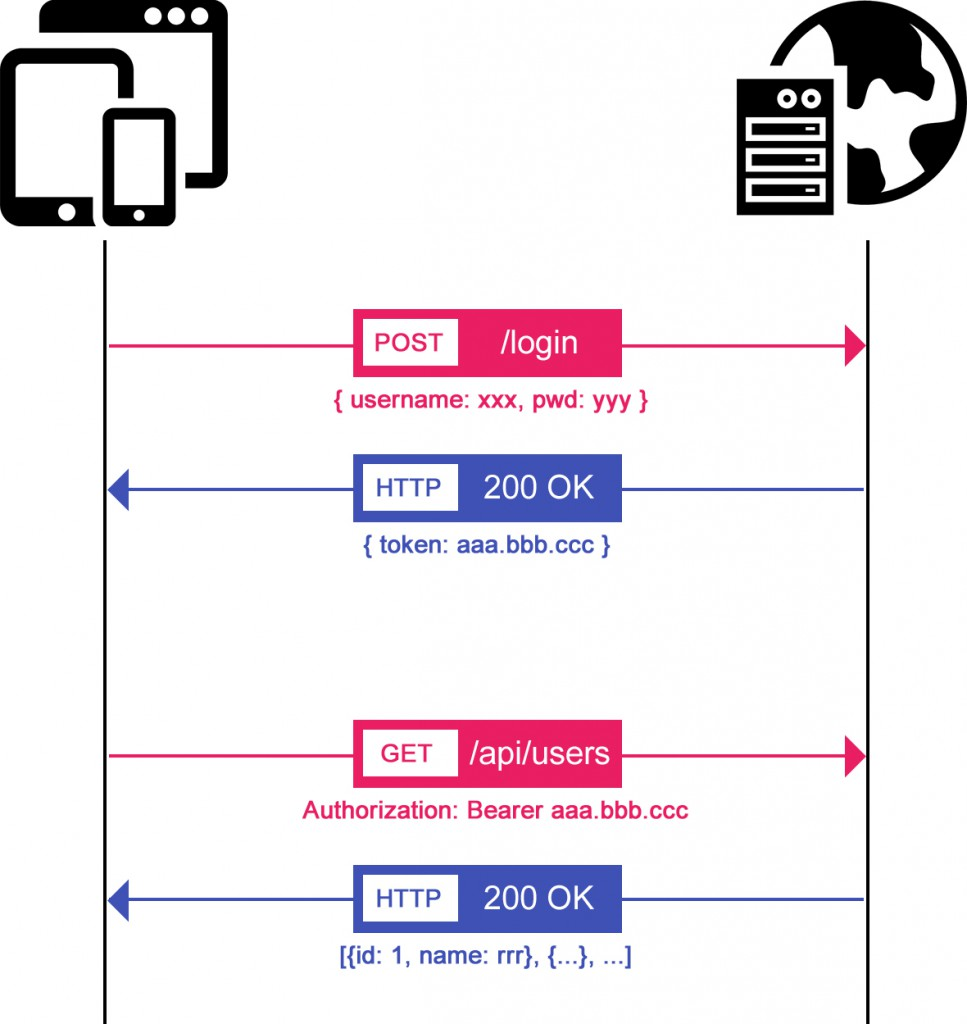
\includegraphics[width=15cm, height=10cm]{img/jwt-token.jpg}
\caption{Schéma de la récupération et de l'utilisation du JWTToken}
\end{figure}

\subsubsection{Le flux RSS de IceScrum et Jira}

IceScrum et Jira bénéficient tous deux de flux RSS. Un flux RSS est un flux continue d'information au format XML qui donnent les dernières modifications sur le site. Par exemple : X a créé une User Story. En triant les données depuis le flux RSS nous pourrons donc récupérer toutes les personnes qui ont interagi avec le projet. Il nous reste qu'un seul élément à régler, l'affichage des résultats des votes.  

\subsubsection{Highcharts}

Afin d'afficher les résultats des votes nous souhaitions pouvoir les consulter sur un graphique. Pour cela il existe beaucoup de plugin en JS qui permettent de générer des graphiques. Notre choix c'est orienté vers \href{https://github.com/highcharts/highcharts}{\textbf{Highcharts}}. Highcharts est facile à mettre en place et est toute aussi facile d'utilisation. 

%%TODO : refaire présentation highcharts %%

\subsection{Réalisation}

Nous avons à nouveau séparé le développement de ce projet en deux, le back end et le front end.

\subsubsection{Le back end}

La premier travail fut de récupérer les personnes actives sur un projet. Pour cela nous avons décidé d'utiliser les flux RSS de IceScrum et Jira. Jira bénéficie pour chaque projet d'un flux RSS que l'ont peut trier. Comme pour la documentation de leurs API REST, leur documentation sur les flux RSS est difficile à trouver. Nous nous sommes donc principalement servis des informations sur les forums de Jira afin d'obtenir les fonctions de tri. Nous pouvons donc trier le flux RSS par rapport à la date. Avec celui-ci, nous sommes capable de savoir quelle personne a participé au projet durant le mois précédent. Ainsi, nous pouvons sélectionner ces personnes pour leurs envoyer le mail de satisfaction. Petite surprise agréable, dans le flux RSS de Jira, l'utilisateur est dans sa propre balise XML ce qui nous donne toutes les informations de cet utilisateur. Cela facilite énormément le travail et nous évite de renvoyer une requête vers le serveur pour récupérer les informations de l'utilisateur.

Pour IceScrum, le flux RSS ne possède pas de documentation et je n'ai pas trouvé de discussion autour. Nous avons donc un flux brut d'informations que nous ne pouvons pas trier. Deuxième surprise, les données du flux RSS ne sont pas conservées. En fonction de l'action effectuée, l'action reste entre 3 heures et 3 mois dans le flux RSS. Nous n'avons donc pour le moment pas mis en place de moyen pour pallier à ce problème. Une solution serait de lancer une tâche cron qui récupère les utilisateurs actifs de IceScrum toutes les 2 heures et les stockent dans la base de données. Nous devons en plus lire la chaîne de caractère afin de récupérer le nom et le prénom de l'utilisateur. Et à partir de ce nom et prénom, nous pouvons faire une requête vers l'API Rest pour récupérer son mail.

Maintenant que nous pouvons récupérer le mail des utilisateurs, nous avons demandé à un membre de l'équipe Design de nous donner un template de mail. Nous avons essayer de faire une vue pour les mails client la plus proche de ce template. Un problème survient, sur navigateur le mail possède le bon design mais pas sur l'application Outlook(application utilisée par la majorité des personnes travaillant dans la SNCF). Afin que Outlook affiche correctement les mails, il faut utiliser des tables HTML ce qui ne facilite pas la mise un place du template de CSS. Malgré tous cela, nous arrivons à mettre en place le template. 

Une fois ces deux flux traités, le mail prêt, nous nous sommes occupés de créer la commande Symfony ainsi que la tâche cron. La commande Symfony fut rapide à préparer, en une classe PHP le problème fut réglé. La tache cron par contre est bien plus compliquée à mettre en œuvre. Afin de la préparer sur tous les environnement disponible (Développement, Intégration, Production) nous avons installer cron sur le Docker. De plus en installant la tâche cron sur le docker, nous n'avons pas à installer PHP pour exécuter la commande Symfony sur le serveur. La commande sera donc effectuée depuis l'intérieur du docker PHP. 

Un autre point important est soulevé à ce moment. Pour pouvoir voter sur notre application, le client arrive sur Metrit et écrit son vote. Nous ne souhaitons pas qu'il est accès à tous la plate-forme. Pour cela nous allons utiliser le Bundle LexikJWTAuthentificationBundle afin de créer un système de connexion dans le front. 

\subsubsection{Le front}

Nous avons commencé par la partie design pour le front. L'équipe design nous a fourni un template de page web avec le code correspondant.

Cette partie nous a paru extrêmement importante. Si un client clique sur le mail pour donner sa satisfaction, mais que lorsqu'il arrive sur Metrit il est accueilli par du HTML sans CSS, il ne risque pas de voter. Nous en avons profité, pour ajouter une option permettant au client de laisser un commentaire. Cela permettra plus tard de comprendre les notations des clients. 

Une fois cette partie design finie, nous avons du implémenter la connexion sur le front. Pour cela, il suffit de modifier le service effectuant préparant les requêtes créé auparavant. 

Vient ensuite la création d'une vue pour les administrateur. L'affichage des votes en fonction des projets. Dans un premier temps nous avons utilisés Highcharts afin d'obtenir un graphique des votes :
\begin{figure}
\centering
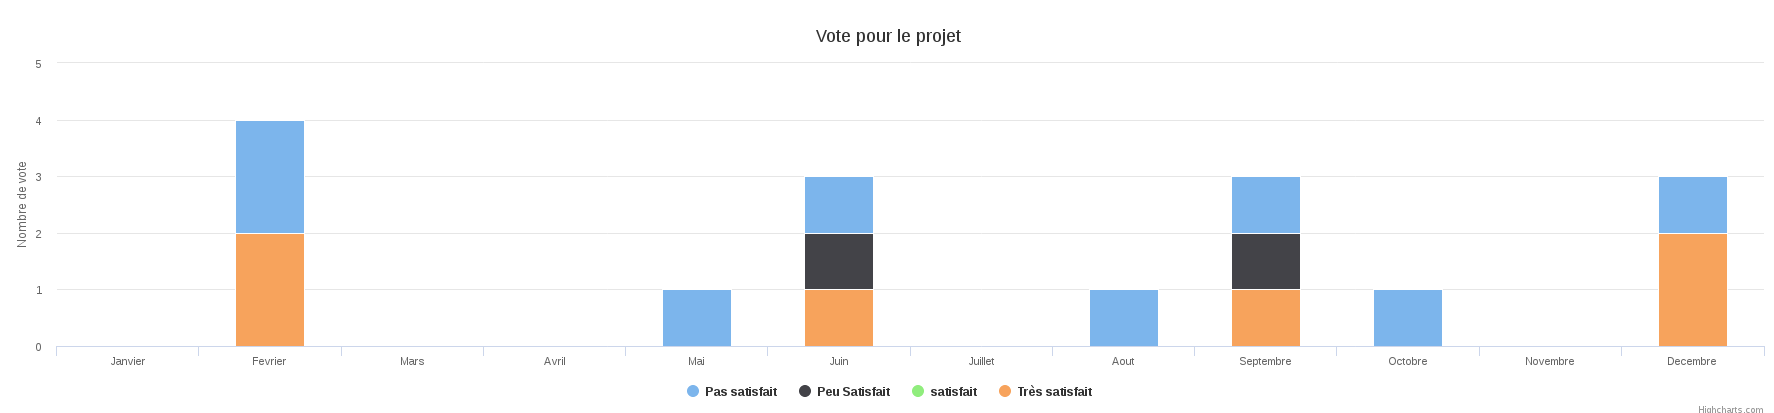
\includegraphics[width=17cm, height=7cm]{img/graphique-high-chart.PNG}
\caption{Graphique Highcharts comprenant des votes}
\end{figure}

Nous avons eu un retour client dessus. L'affichage est bien détaillé, mais dans l'idéal, le client voudrait une deuxième vue avec un tableau si possible. Nous avons donc ajouté à notre application un deuxième onglet comprenant les statistiques simplifiés dans un tableau. 

\subsection{Amélioration possible}

Nous avons plusieurs axes d'améliorations possible pour ce projet. Dans un premier temps il n'existe qu'un seul compte administrateur stocké dans les variables d'environnement. Il est envisageable de faire un système de compte utilisateur qui soit stocké dans la base de données. Cela permettrait d'avoir plus de possibilité sur les rôles par exemple. Ensuite cela éviterais d'avoir un seul compte partagé avec toutes l'entreprise.

Un second axe d'amélioration pour ce projet serait de générer plus de log. Pour l'instant les seuls logs qui sont générés sont ceux de Symfony. Il pourrait être intéressant d'avoir plus de logs notamment sur la tâche cron. Pour le moment on ne peut pas être sûre que la tâche se soit effectuée. Même si elle a été testée en environnement de développement, nous n'avons pas encore envoyer de mail depuis le serveur de production. Le seul moyen sans logs, de savoir si la tâche s'est bien effectuée, est de voir si un client à bien répondu au mail de satisfaction. Cela n'est pas viable pour pouvoir valider le fonctionnement de l'application.

\chapter{Conclusion}

\section{Bilan des applications}

Metrit et ses deux applications répondent donc aux besoins de Itnovem. Le générateur de mail permet de gagner du temps lors des fins de sprint et d'avoir un mail standardisé dans tous les projets de Itnovem. 

Malgré un besoin commun à beaucoup de développeurs, le générateur de mail de fin de sprint n'a jamais été partagé en open source. Il s'agit pourtant d'un élément clé pour la communication entre l'équipe de développeurs et les clients. Sur Trello, cela reste compréhensible car l'application n'a pas pour objectif premier la gestion de projet. Mais pour IceScrum ainsi que Jira ces deux applications ont pour cœur de métier la gestion de projet. Il paraît étonnant qu'il n'y ait pas la possibilité de générer des mails de fin de tâches/sprint pour des projets. 

Notre solution apporte un mail standard, dans une application simple à utiliser.  D'un point de vue technique, elle n'est pas très complexe. Le point le plus difficile de l'application fut la compréhension des outils de gestion de projet. 

L'application de satisfaction client par contre est beaucoup plus commune. Il existe énormément de moyen de générer un questionnaire pour obtenir la satisfaction d'un client. Un simple Google Forms pourrait suffire. Ce qui est plus intéressant dans cette application fut la récupération des utilisateurs concernés ainsi que l'automatisation du processus.

\section{Bilan personnel}

Ce stage m'a permis d'enrichir mes connaissances du milieu de l'entreprise. J'ai découvert énormément de techniques de programmation qui sont plus utilisées dans le milieu de l'entreprise. Par exemple, la mise en place de variables d'environnements est une des difficultés que j'ai toujours eues. Durant ce stage j'ai énormément interagi avec des variables d'environnements, j'ai même découvert qu'angular pouvait aussi simuler des variables d'environnement. 

Angular possède un système qui permet de build le projet en fonction de l'environnement du projet (production, intégration, développement ...). Il permet d'avoir des variables spécifiques à ces environnement. Il s'agit d'un autre point clé de ce que j'ai appris pendant le stage. Je n'avais jamais effectué de la gestion de plusieurs environnement auparavant. J'appréhendais énormément mais grâce à Hamouda j'ai pu mieux comprendre comment organiser les environnements. 

En organisation de projet aussi, j'ai appris beaucoup de choses. La plus importante fut l'utilisation de services. Après mon premier sprint Hamouda m'a demandé de refactorer mon code afin d'utiliser un maximum les services. Il s'agit de classes qui contiennent du code qui pourrait être réutilisé. Le contrôleur ne contient donc que très peu de code et uniquement des appels vers des fonctions de services. Cela m'a permit de mieux organiser mon code. 

J'ai pu aussi découvrir Symfony en tant que technologie web ainsi que de rattraper mon retard sur les versions d'Angular.

De plus avec les méthodes employées dans l'entreprise, ainsi que l'utilisation d'outil de gestion de projets agiles, j'ai pu élargir mon apprentissage des méthodes agiles.

\section{Webographie}

Consulté le 16/06/2018 : documentation API Rest IceScrum

https://www.icescrum.com/documentation/rest-api/ \\

Consulté le 16/06/2018 : documentation API Rest Jira 

https://developer.atlassian.com/cloud/jira/platform/rest/ \\

Consulté le 16/06/2018 : documentation API Rest Trello

https://trello.readme.io/docs/api-introduction \\

Consulté le 16/06/2018 : Post sur l'arrêt de l'entretiens de l'API SOAP de mantisBT

https://support.mantishub.com/hc/en-us/articles/203574999-MantisHub-SOAP-API \\

Consulté le 17/06/2018 : Récupération de l'information sur le nombre de développeurs de la communauté.

https://symfony.com/community \\

Consulté le 18/06/2018 : Documentation sur le Bundle Symfony Doctrine

https://symfony.com/doc/current/doctrine.html \\

Consulté le 18/06/2018 : Documentation sur le Bundle Symfony SwiftMAilerBundle

https://symfony.com/doc/current/email.html \\

Consulté le 18/06/2018 : Documentation sur la console de Symfony

https://symfony.com/doc/current/console.html \\

Consulté le 18/06/2018 : Documentation sur le Bundle LexikJWTAuthenticationBundle

https://github.com/lexik/LexikJWTAuthenticationBundle \\

Consulté le 18/06/2018 : Documentation sur le WYSIWIG utilisé dans le front

https://github.com/Sibiraj-S/ngx-editor \\

Consulté le 18/06/2018 : Documentation sur le package Cron 

https://doc.ubuntu-fr.org/cron \\

Consulté le 16/06/2018. Récupération de l'image pour décrire le fonctionnement du front/back end

https://blog.octo.com/les-nouvelles-architectures-front-web-et-leur-impact-sur-la-dsi-partie-2/ \\

Consulté le 19/06/2018. Récupération de l'image pour décrire l'échange des JWT token.

https://www.ekino.com/introduction-aux-json-web-tokens/%% => image 


\printbibliography[heading=bibintoc]

\tableofcontents

\end{document}